
\label{subsec:ANN:perceptron}

Perceptrons are the simplest topology we can build with artificial neurons. 
Nevertheless, the knowledge of the operations behind perceptrons provides a good
basis for understanding more complex networks.

A perceptron neuron uses the hard-limit activation function, which produces a 1 if the net input is equal to or greater than 0; otherwise it produces a 0. 
This function gives a perceptron the ability to classify input vectors by dividing the input space into two regions, which are formed by the decision boundary line L at $\mathbf{Wp} + b = 0$ \cite{demuth2008neural}. 
This line is perpendicular to the weight matrix W and shifted according to the bias b 
(notice that hard-limit neurons without a bias will always have a classification line going through the origin).

As shown in \figref{perceptron}, the perceptron network consists of a single layer of 
$S$ perceptron neurons connected to $R$ inputs through a set of weights $\mathbf{W}$.

\begin{figure}[!ht]
\centering
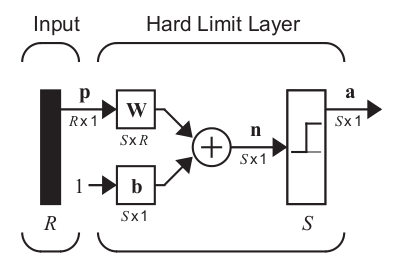
\includegraphics[width=0.5\textwidth]{images/perceptron.png}
\caption{Perceptron network}
\label{fig:perceptron}
\end{figure}



